\problem{Forced Equations and Resonance}

This homework investigates spring equations using the following code, which has been slightly modified to use correct variable names:

\begin{verbatim}
function LAB6
omega0 = 2; c = 1; omega = 1.4;
param = [omega0,c,omega];
t0 = 0; y0 = 0; v0 = 0; Y0 = [y0;v0]; tf = 50;
options = odeset('AbsTol',1e-10,'RelTol',1e-10);
[t,Y] = ode45(@f,[t0,tf],Y0,options,param);
y = Y(:,1); v = Y(:,2);
figure(1)
plot(t,y,'b-'); ylabel('y'); grid on;
t1 = 25; i = find(t>t1);
C = (max(Y(i,1))-min(Y(i,1)))/2;
disp(['computed amplitude of forced oscillation = ' num2str(C)]);
Ctheory = 1/sqrt((omega0^2-omega^2)^2+(c*omega)^2);
disp(['theoretical amplitude = ' num2str(Ctheory)]);
function dYdt = f(t,Y,param)
y = Y(1); v = Y(2);
omega0 = param(1); c = param(2); omega = param(3);
dYdt = [ v ; cos(omega*t)-omega0^2*y-c*v ];
\end{verbatim}

Originally, this generates the following plot:

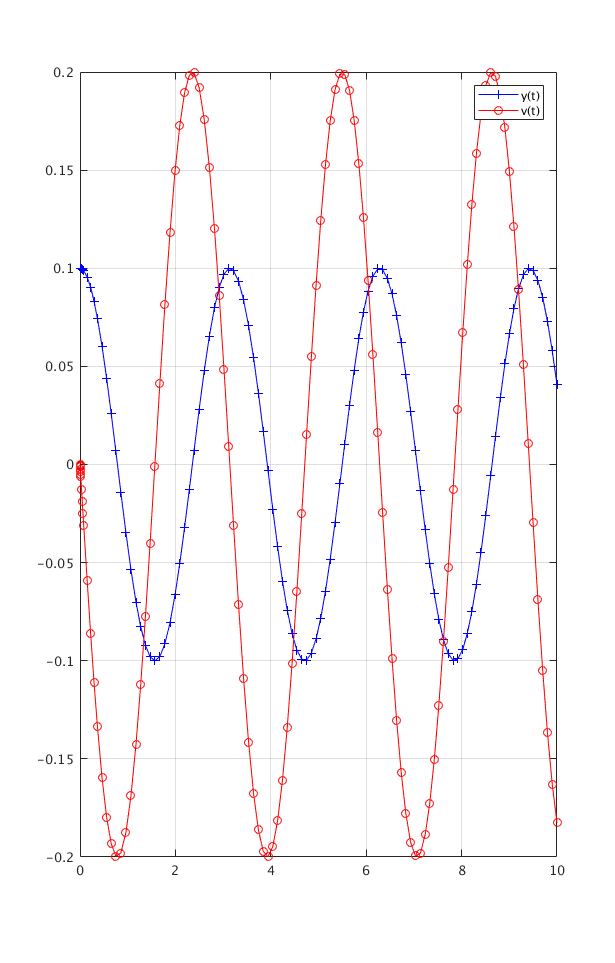
\includegraphics[scale=0.4]{0.png}

\solution
\part
What is the period of the forced oscillation? What is the numerical value (modulo $2\pi$) of the angle $\alpha$ defined by (L6.4)?

%Since the frequency is known ($\omega = \sqrt{\omega_0^2 - \frac{c^2}{4}} = \sqrt{4 - \frac{1}{4}} = \sqrt{15/4}$), the period is the inverse of this, or $\frac{1}{\sqrt{15/4}}$ seconds, which can be verified on the graph included.
Since the frequency is known ($\omega = 1.4$), the period is the inverse of this, or $0.7143$ seconds/radian, which can be verified on the graph included (as 4.487 seconds, roughly, which is $2\pi * 0.7143$).
Since $\omega < \omega_0$, $\alpha$ is $arctan(\frac{c\omega}{\omega_0^2 - \omega^2})$, or $arctan(\frac{\sqrt{15/4}}{4 - 15/4}) = 0.451$.

\part
Modify the above code to plot the complementary solution of (L6.1), that is, the first term in (L6.2). First define in the file the angle $\alpha$ using (L6.4), then evaluate the complementary solution $y_c$ by subtracting the quantity $C cos(\omega t − \alpha)$ from the numerical solution $y$. Plot the resulting quantity. Does it look
like an exponentially decreasing oscillation? Why or why not? Include the modified M-file
and the corresponding plot.

The modified code is posted below. It adds an $\alpha$ calculated and $y_c$ calculation. Based on the plot, the $y_c$ is certainly exponentially decreasing, because it decreases\ldots exponentially, where the previous plot showed (seemingly) stability after an initial period. This is because the exponential portion of the equation approaches zero, while $C cos(\omega t - \alpha$) is a typical (stable, non dampening) $cos$ function (with scaling, stretching, and translation), much like in the very first example
    discussed in class, $x - y$. So if the second part of $y$ is removed, then the exponentential portion simply goes to zero (because the power is negative).

\begin{verbatim}
function LAB6
omega0 = 2; c = 1; omega = 1.4; a = 0;
if omega0 > omega
    a = atan((c * omega) / (omega0 * omega0 - omega * omega))
else
    a = atan((c * omega) / (omega0 * omega0 - omega * omega)) + 3.1415
end
param = [omega0,c,omega,a];
t0 = 0; y0 = 0; v0 = 0; Y0 = [y0;v0]; tf = 50;
options = odeset('AbsTol',1e-10,'RelTol',1e-10);
[t,Y] = ode45(@f,[t0,tf],Y0,options,param);
y = Y(:,1); v = Y(:,2);
t1 = 25; i = find(t>t1);
C = (max(Y(i,1)) - min(Y(i,1))) / 2;
y = y - C * cos(omega * t - a)
figure(1)
plot(t,y,'b-'); ylabel('y'); grid on;
disp(['computed amplitude of forced oscillation = ' num2str(C)]);
Ctheory = 1/sqrt((omega0^2-omega^2)^2+(c*omega)^2);
disp(['theoretical amplitude = ' num2str(Ctheory)]);

function dYdt = f(t,Y,param)
y = Y(1); v = Y(2);
omega0 = param(1); c = param(2); omega = param(3); a = param(4);
dYdt = [ v ; cos(omega*t)-omega0^2*y-c*v ];

\end{verbatim}

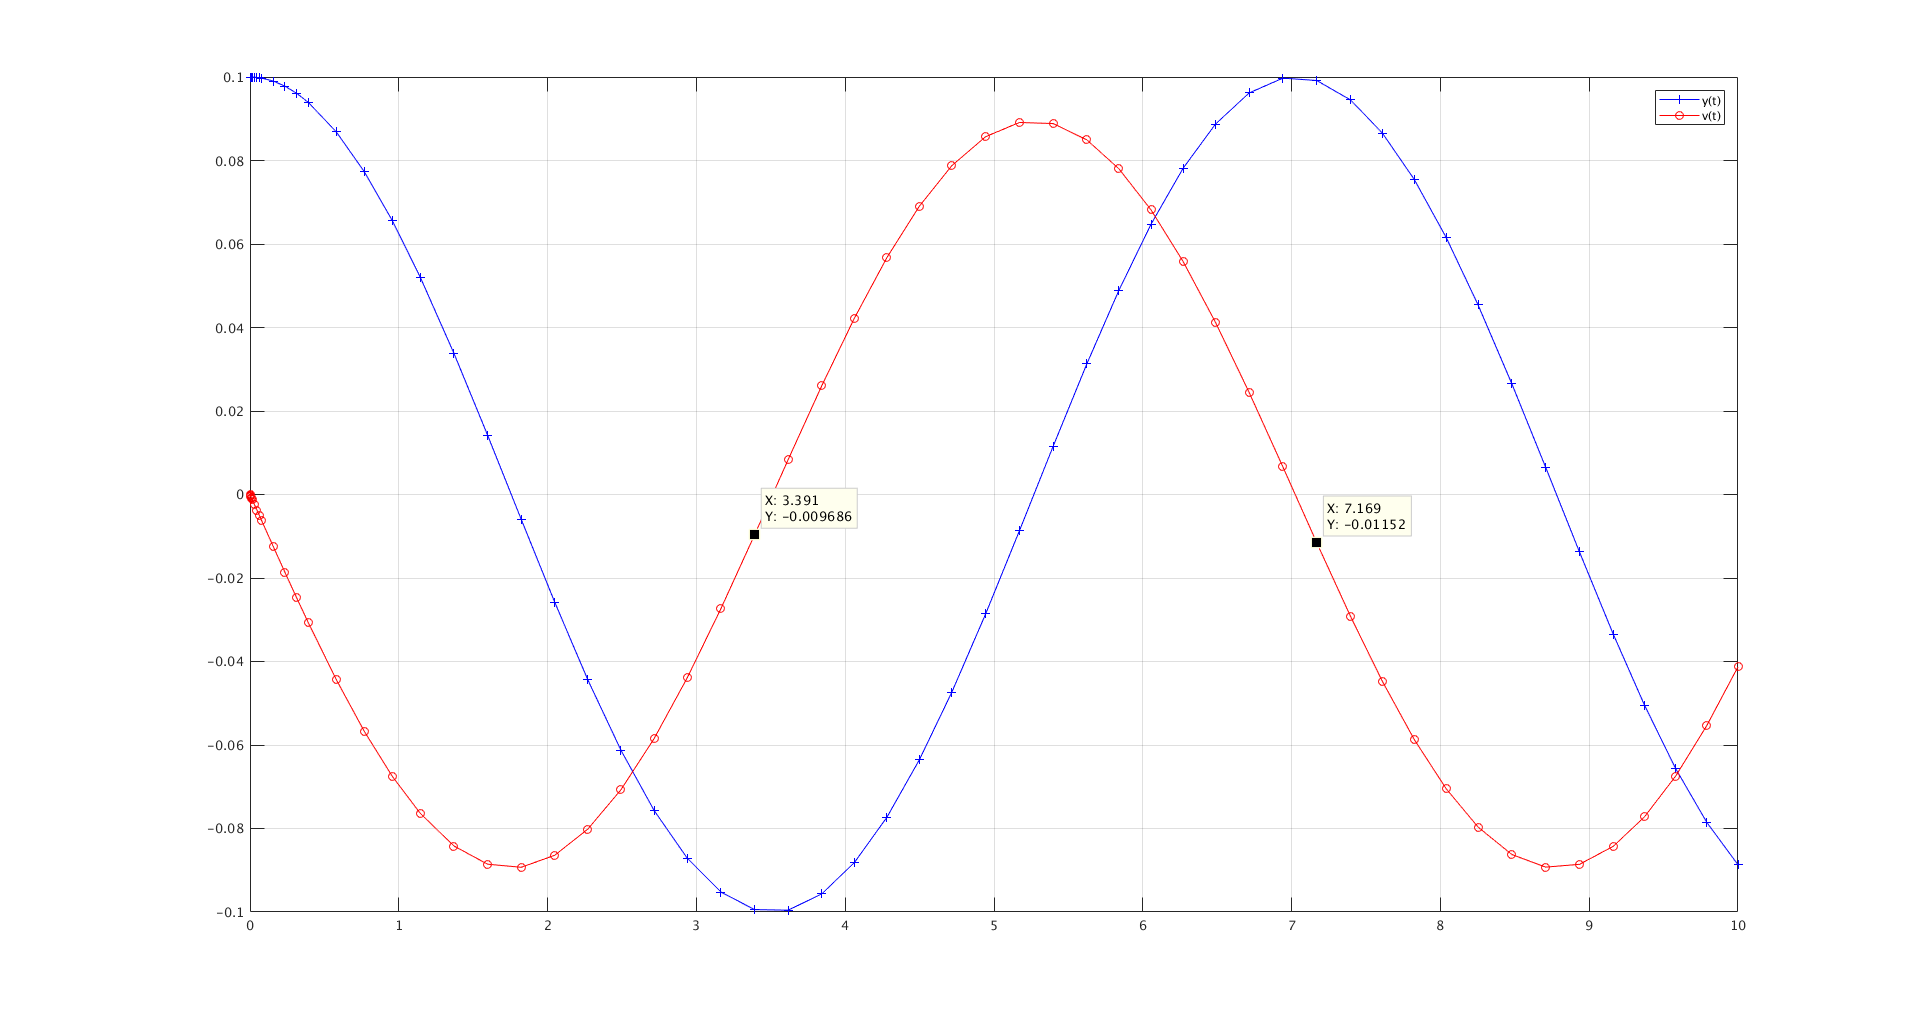
\includegraphics[scale=0.4]{1.png}
